\documentclass[aspectratio=169]{beamer}


\makeatletter
\newlength\beamerleftmargin
\setlength\beamerleftmargin{\Gm@lmargin}
\makeatother

%%%%%%% STYLE %%%%%%%%%%%%%%%%%%%%%%%%%%%%%%%%%%%%%%%%%%%%
% FONTS
\usepackage[proportional]{sourcesanspro}
\usepackage[T1]{fontenc}

\usepackage{soul}   % Rayer

% Rayer a un certain moment seulement
\newcommand<>{\sta}[1]{
  \alt#2{\st{#1}}{{#1}}
}


\usepackage{hyperref}
\usepackage{multirow}

% TITLE
\setbeamerfont{frametitle}{size=\large}


% MARGINS
\newenvironment{changemargin}[2]{%
  \begin{list}{}{%
    \setlength{\topsep}{0pt}%
    \setlength{\leftmargin}{#1}%
    \setlength{\rightmargin}{#2}%
    \setlength{\listparindent}{\parindent}%
    \setlength{\itemindent}{\parindent}%
    \setlength{\parsep}{\parskip}%
  }%
  \item[]}{\end{list}} 

% FOOTNOTES
\renewcommand{\thefootnote}{}
\renewcommand{\footnoterule}{}

% MATHS
\usepackage{amsmath, amssymb, amsfonts}
%\usepackage[OMLmathrm,OMLmathbf]{isomath}

% LISTS
%\usepackage{enumitem}

% Enumerate style
\setbeamertemplate{enumerate items}[circle]
\setbeamercolor{item projected}{bg=maincol,fg=bgcol}

\setbeamertemplate{itemize subitem}{\color{maincol}$\blacktriangleright$}
\setbeamertemplate{itemize item}{\color{maincol}$\blacktriangleright$}

% Description
\setbeamercolor{description item}{ fg=maincol}

% COLORS
\usepackage{xcolor}
%\input{~/Dropbox/Presentations/Templates/tangocolors.sty}

\definecolor{bgcol}{rgb}{1,1,1} % Background color
\definecolor{fgcol}{rgb}{0,0,0} % Foreground color

\definecolor{maincol}{RGB}{0, 107, 137} % Bleu canard %006b8b
\definecolor{col1}{RGB}{125, 72, 150} % Purple %7d4896
\definecolor{col2}{RGB}{178, 208, 76} % Light green %b0d04c

\definecolor{col12A}{RGB}{169, 152, 100}
\definecolor{col12B}{RGB}{42, 117, 125}

%\definecolor{maincol}{HTML}{7D1935} % Rubis
%\definecolor{col1}{HTML}{4A96AD} % Blue
%\definecolor{col2}{HTML}{575042} % Brown

\definecolor{cl1}{HTML}{234BCD}
\definecolor{cl2}{HTML}{5D5B8F}
\definecolor{cl3}{HTML}{976C52}
\definecolor{cl4}{HTML}{D17D15}

\definecolor{mgray}{gray}{0.55}
\definecolor{dgray}{gray}{0.3}
\definecolor{lgray}{gray}{0.75}
\definecolor{gray70}{gray}{0.70}

% COLORS AND THEMES
\usecolortheme[named=maincol]{structure} 
\setbeamercolor{alerted text}{fg=maincol} 
\setbeamercolor{frametitle}{fg=maincol}
\setbeamercolor{structure}{fg=fgcol, bg=bgcol}



% TITLE SECTION
\newcommand{\titlesec}[3]{\begin{center}
  \vspace{1.5cm}
                           \parbox{0.8\textwidth}{\textcolor{#3}{\begin{center} \Large #1 \\ \vspace{0.75cm} {\small \textcolor{mgray}{#2}} \end{center}}} \end{center}
			  }

% DESSINS
%\usepackage{pgf}
\usepackage{tikz}

\usetikzlibrary{patterns}
\usetikzlibrary{positioning,shadows,backgrounds,decorations.pathreplacing}
\usetikzlibrary{fit, calc}
\usetikzlibrary{shapes, shapes.callouts, decorations.text}
\usetikzlibrary{arrows}
%\usepackage{pgfplots}
\usepackage{rotating}

% GENERAL LAYOUT
\setbeamertemplate{navigation symbols}{} 
\setbeamertemplate{blocks}[rounded][shadow=false]

\setbeamercolor*{author in head/foot}{parent=palette quaternary}
\setbeamercolor*{title in head/foot}{parent=palette quaternary}
\setbeamercolor*{date in head/foot}{parent=palette quaternary}
\setbeamercolor*{section in head/foot}{fg=mgray}
\setbeamercolor*{subsection in head/foot}{parent=palette quaternary}

\def \hbarfoot {2.5ex}
\def \dbarfoot {1.75ex}
\defbeamertemplate*{footline}{infolines theme}
{
  \leavevmode%
  \hbox{%
  %
  \begin{beamercolorbox}[wd=.33\paperwidth, ht=\hbarfoot, dp=\dbarfoot, center]{section in head/foot}%
    \usebeamerfont{author in head/foot}
    \insertshortauthor % Uncomment to add author's name in the foot
      \end{beamercolorbox}
      %
  \begin{beamercolorbox}[wd=.33\paperwidth, ht=\hbarfoot, dp=\dbarfoot, center]{section in head/foot}%
    \usebeamerfont{title in head/foot}
% ESEB, August 2017
  \end{beamercolorbox}%
  %
  \begin{beamercolorbox}[wd=.33\paperwidth, ht=\hbarfoot, dp=\dbarfoot, right]{bg=bgcol, fg=fgcol}%
    \usebeamerfont{date in head/foot}
    \insertframenumber{} %/ \inserttotalframenumber %
	\hspace*{2ex} 
  \end{beamercolorbox}}%
  \vskip0pt%
}


\addtobeamertemplate{footline}{%
  %\leavevmode%
  \color{maincol!50!white}% to color the progressbar
%  \hspace*{-\beamer@leftmargin}%
%  \rule{\beamer@leftmargin}{2pt}%
  \rule{\dimexpr \insertframenumber\paperwidth/\inserttotalframenumber}{\dimexpr -1.25pt+\dbarfoot}
  % next 'empty' line is mandatory!

%  \vspace{0\baselineskip}
\vspace{\dimexpr -\hbarfoot-\dbarfoot}
  {}
}


% BLOCKS

%\addtobeamertemplate{block begin}{\pgfsetfillopacity{0.}}{\pgfsetfillopacity{1}}
%\addtobeamertemplate{block beamercolorbox begin}{\pgfsetfillopacity{0.65}}{\pgfsetfillopacity{1}}
%\setbeamercolor{block title}{fg=maincol, bg=red}%use=structure,fg=black,
%     bg=white!10}
\setbeamercolor{block title}{bg=white!10, fg=maincol}
%\setbeamercolor{block body}{%use=structure,fg=black,
%     bg=white!10}
\setbeamerfont{block title}{size=\normalsize}



\newcommand{\smallblock}[3]{
\begin{minipage}[c]{#1}
  \begin{block}{#2}
   #3
  \end{block}
\end{minipage}
}





% ROTATE TEXT FOR CREDITS
\usepackage{graphics}
\definecolor{lgray}{gray}{0.75}
\newcommand{\piccredit}[1]{\hspace{0.1em}\rotatebox{90}{\tiny \textcolor{gray70}{(c) #1}}}
\newcommand{\picc}[1]{ \rotatebox{90}{\tiny \textcolor{lgray}{#1}}}

% STROKE
%\usepackage{ulem}

% TABLES
\usepackage{array}

% ANIMATIONS - MOVIES
\usepackage{multimedia}


\newcommand{\refpaper}[3]{
\begin{flushright}
\textcolor{gray50}{\tiny #1 (#2), \textit{#3}}
\end{flushright}
}

%% Maths

%\newcommand{\mat}[1]{\mathrm{\mathbf{#1}}}
\newcommand{\mat}[1]{\mathbf{#1}}
\DeclareMathOperator{\Tr}{Tr}
\newcommand{\Trace}[1]{\Tr \left( #1 \right)}

%% Command for Raising pictures
\newcommand{\raisepic}[1]{\raisebox{-\height}{#1}}
\newcommand{\midpic}[2]{\raisebox{-#2\height}{#1}}

% Checkmarks
\usepackage{pifont}
\newcommand{\cmark}{\ding{51}}%
\newcommand{\xmark}{\ding{55}}%



% REFERENCES
%% References
\newcommand{\pprref}[2]{\textcolor{mgray}{#1 (#2)}}
%\usepackage{natbib}
% Remove the icon before each item
\setbeamertemplate{bibliography item}{}

% Only number References slides if they are more than 1
\setbeamertemplate{frametitle continuation}[from second]

%remove line breaks
\setbeamertemplate{bibliography entry title}{}
\setbeamertemplate{bibliography entry location}{}
\setbeamertemplate{bibliography entry note}{}

%\setbeamercolor*{bibliography entry title}{fg=fgcol}
\setbeamercolor*{bibliography entry author}{fg=maincol}
%\setbeamercolor*{bibliography entry note}{fg=fgcol}
%\setbeamercolor*{bibliography entry location}{fg=fgcol}


% In text?
\newcommand{\refstyle}[1]{\scriptsize  \textcolor{dgray}{#1}}

% As footnote
\newcommand{\theref}[1]{{\footnotetext{\begin{flushright} \refstyle{#1} \end{flushright} } }}

% NOTES
%\setbeamertemplate{note page}[plain]
\setbeamerfont{note page}{size=\scriptsize}

% APPENDIX
% Change numbering for the appendix
\newcommand{\backupbegin}{
   \newcounter{framenumberappendix}
   \setcounter{framenumberappendix}{\value{framenumber}}
}
\newcommand{\backupend}{
   \addtocounter{framenumberappendix}{-\value{framenumber}}
   \addtocounter{framenumber}{\value{framenumberappendix}} 
}

% HYPERLINKS
\setbeamercolor{button}{bg=maincol,fg=bgcol}

% DESCRIPTIONS
\defbeamertemplate{description item}{align left}{\insertdescriptionitem\hfill}


\newcommand{\btVFill}{\vskip0pt plus 1filll}
\newcommand{\EE}{\mathbb{E}}
\newcommand{\PP}{\mathbb{P}}

%%%%%%%%%%%%%%%%%%%%%%%%%%%%%%%%%%%%%%%%%%%%%%%%%%%%%%

%\colorlet{colA}{ta2chameleon}
%\colorlet{colB}{ta2chocolate}

% Colors for the legends
\definecolor{pinka}{HTML}{DA8DAC}
\definecolor{pinkb}{HTML}{ac0045}
\definecolor{pinkc}{HTML}{4c001e}
\definecolor{pinkd}{HTML}{ecc6d5}


%\newcommand{\sderivv}[3]{\left.\frac{\partial #1}{\partial #2}\right|_{#3 =0}}
\newcommand{\sderivv}[3]{\left. \frac{\partial #1}{\partial #2} \right|_{\delta =0}}

\newcommand{\ssum}[2]{{\textstyle \sum\limits_{#1}^{#2}}}

\newcommand{\bb}{\mathsf{b}}
\newcommand{\cc}{\mathsf{c}}
\newcommand{\dd}{\mathsf{d}}

\begin{document}

% TITLE PAGE
\begin{frame}
\begin{center}
Symposium 9: Fitness and evolution in a social environment: from theory to reality

\vspace{1em}

\begin{tikzpicture}
\node[text width=0.8\textwidth, font=\Large, align=center, color=maincol](tit){Fidelity of parent-offspring transmission\\ and the evolution of social
\mbox{behavior} in subdivided populations.};

\tikzstyle{nameauthor}=[inner sep=2pt, draw=none, anchor=base]
\def \dhn {2.25cm}
\node[below=2em of tit, nameauthor](FD){F. D\'ebarre};

\node[below=-0.35cm of FD](sFD){}; % Removing pic because looks odd with single author
\tikzstyle{twee}=[font=\footnotesize, minimum height=2em]
\node[below=0cm of sFD, twee](tFD){@flodebarre};
\node[left=0cm of tFD]{\includegraphics[height=1em]{/home/florencedebarre/Dropbox/Presentations/GlobalPics/twitter.pdf}};
\end{tikzpicture}

{\footnotesize CNRS \\ Centre de Recherches Interdisciplinaires en Biologie, Paris}

\vspace{1em}

\vfill

%    \hspace*{-\beamerleftmargin}%
\includegraphics[width=0.8\textwidth]{Pics/headerESEB.pdf}
\end{center}
\end{frame}


\section{Results}
\begin{frame}<1-8>[label = EXframe]{Expected frequency of altruists in the population}
\begin{center}
\begin{tikzpicture}[node distance = 0.2cm and 0.16cm, anchor = base, baseline = 0pt]
% vertical and horizontal
\tikzstyle{math}=[font=\large, inner sep = 0pt, draw = none, minimum height = 1.2cm]

\def \blsk {-1em}

\node[math, anchor = west] (EX) at(0,0){$\mathbb{E}[\overline{X}]$};
\node[math, right = of EX] (equal){$=$};
\node[math, right = of equal](nu){$\nu$};
\node[math, right = of nu](plus){$+$};
\node[math, right = of plus](sel){$\selstr$};
\node[math, right = of sel](nuvar){$\nu (1-\nu)$};
\node[math, right = of nuvar](fac){$\dfrac{1-\mu}{\mu}$};
\node[math, right = of fac](fact){$\left(1 - \Qout \right)$};
\node[math, right = of fact]{$\times$};
\node[math, below = of plus] (blocCD){$-c$};
\node[math, left = of blocCD]{$\Bigg($};
\node[math, right = of blocCD] (blocCI){$- \, (b - c) \left( \dfrac{(1-m)^2}{\demesize} + \dfrac{m^2}{\demesize \, (\nbdemes - 1)} \right)$};
\node[math, below = of blocCD.south west, anchor = north west](pluss){$+$};
\node[math, right = of pluss](R){$ \dfrac{\Qin - \Qout}{1 - \Qout}$};
\node[math, right = of R](lbrace){$\Bigg[$};
\node[math, right = of lbrace](blocBD){$b$};
\node[math, right = of blocBD](blocBI){$- \, (b-c) \, (n-1) \, \left( \dfrac{(1-m)^2}{\demesize} + \dfrac{m^2}{\demesize \, (\nbdemes - 1)} \right)$};
\node[math, right = of blocBI](rbrace){$\Bigg]$};
\node[math, right = of rbrace]{$\Bigg)$};

\tikzstyle{highlgt}=[rectangle, rounded corners = 2pt, line width = 1pt, fill opacity = 0.4, text height = 0.5cm, fill = maincol, draw = none, inner sep = 0.5pt]
\tikzstyle{explain}=[font=\normalsize, color = maincol, anchor = north west, align = left, inner sep = 1pt, font = \small]
\tikzstyle{lnk}=[draw = maincol, line width = 1.5pt]


\begin{scope}[on background layer]

\pause

\node[highlgt, fit = (nu)](hnu){};
\node[explain] at (0, 2) (enu){Mutation-drift\\equilibrium};
\path[lnk](hnu.north)--(enu);

\pause

\node[highlgt, fit = (sel)](hsel){};
\node[explain] at(2, 1.65)(esel){Selection\\strength};
\path[lnk](hsel.north)--(esel);

\pause

\node[highlgt, fit = (nuvar)](hnuvar){};
\node[explain] at(4, 2)(enuvar){\st{Population variance}\\Variance in the state of one site};
\path[lnk](hnuvar.north)--(enuvar);

\pause

\node[highlgt, fit = (blocCD)(blocCI), fill = col1](hC){};
\tikzstyle{explainH}=[explain, font=\LARGE, anchor = center]
\node[explainH, right = of hC, color = col1]{$-\mathcal{C} \uncover<11->{\nearrow}$};

\pause

\node[highlgt, fit =(blocBD)(blocBI), fill = col2](hB){};
\node[explainH, below = of hB, color = col2]{$\mathcal{B} \uncover<11->{\nearrow}$};

\pause

\node[highlgt, fit = (R), fill = col3](hR){};
\node[explainH, below = of hR, color = col3]{$R \uncover<9->{\searrow}$};

\uncover<12->{
\node[highlgt, fit = (fact), fill = maincol](ht){};
\node[explainH, above = of ht, color = maincol]{$\searrow$};
}

\end{scope}

\uncover<8,9>{
\tikzstyle{blind}=[rectangle, fill = bgcol, fill opacity = 0.9, inner sep = 0pt, rounded corners = 2pt]

\node[blind, fit = (blocBI)]{};
\node[blind, fit = (blocCI)]{};
}

\end{tikzpicture}
\end{center}

\uncover<9>{\phantom{{\Huge X}}}
\end{frame}

\begin{frame}{How does relatedness $R$ change with the emigration probability $m$?}
\pause 

\begin{center}
\begin{tikzpicture}
\node[](pWF){\includegraphics[width = 0.45\textwidth]{../../Programs/R/Pics/ESEB_RplotWF.pdf}};
\node[above = 0cm of pWF]{Wright-Fisher (N deaths)};

\node[right = 0cm of pWF](pM){\includegraphics[width = 0.45\textwidth]{../../Programs/R/Pics/ESEB_RplotM.pdf}};
\node[above = 0cm of pM]{Moran (1 death)};
\end{tikzpicture}
\btVFill 
($\demesize = 4, \nbdemes = 15$)
\end{center}
\end{frame}


\againframe<9->{EXframe}


\def \wpic {0.45\textwidth}

\begin{frame}{Effect of the emigration probability $m$ on the expected proportion of altruists}

\begin{center}
\begin{tikzpicture}
\uncover<1>{
\node[](pWF){\includegraphics[width=\wpic]{{../../Programs/R/Pics/ESEB_EXWF_sel0.005_htg0_justMu0}.pdf}};
}

\node[above = 0cm of pWF]{Wright-Fisher ($N$ deaths \& $N$ births)};

\uncover<2>{
\node[]at(pWF) (pWFp){\includegraphics[width=\wpic]{{../../Programs/R/Pics/ESEB_EXWF_sel0.005_htg0_1}.pdf}};
}
\uncover<3>{
\node[]at(pWF) (pWFp){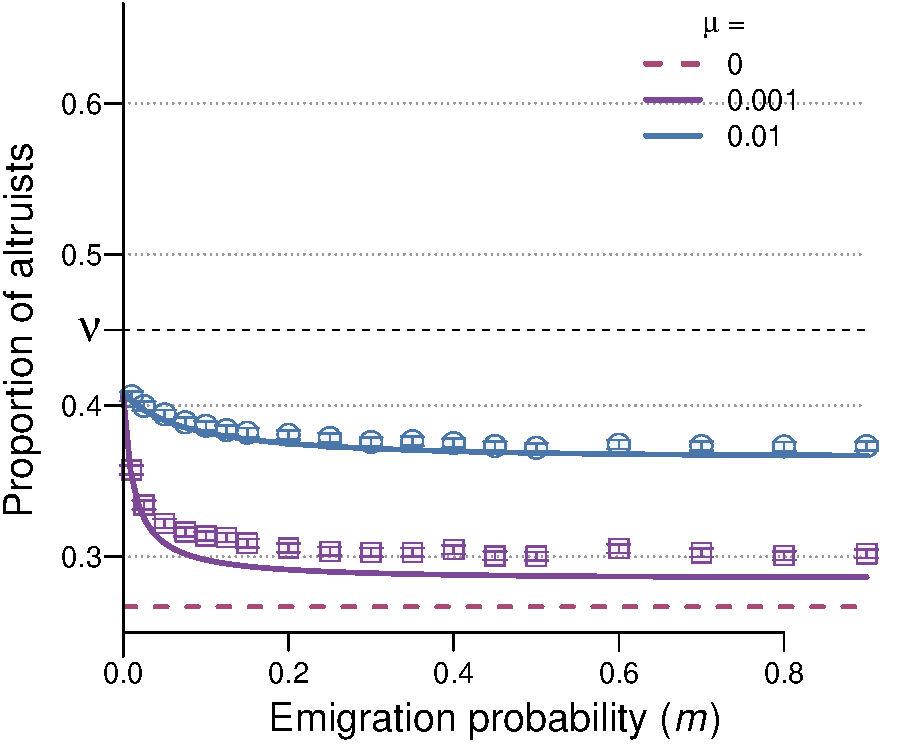
\includegraphics[width=\wpic]{{../../Programs/R/Pics/ESEB_EXWF_sel0.005_htg0_2}.pdf}};
}
\uncover<4>{
\node[]at(pWF) (pWFp){\includegraphics[width=\wpic]{{../../Programs/R/Pics/ESEB_EXWF_sel0.005_htg0_3}.pdf}};
}
\uncover<5->{
\node[]at(pWF) (pWFp){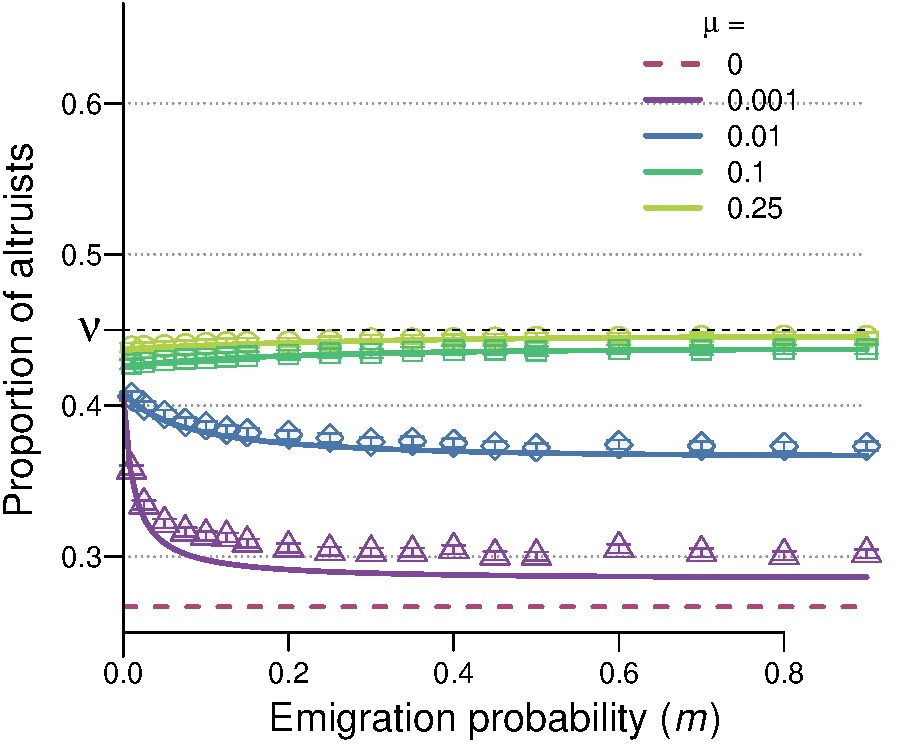
\includegraphics[width=\wpic]{{../../Programs/R/Pics/ESEB_EXWF_sel0.005_htg0_4}.pdf}};
}

\uncover<6>{
\node[right = 1ex of pWF](pM){\includegraphics[width=\wpic]{{../../Programs/R/Pics/ESEB_EXDB_sel0.005_htg0_justMu0}.pdf}};
}
\uncover<6->{
\node[above = 0cm of pM]{Moran Death-Birth ($1$ death \& $1$ birth)};
}
\uncover<7>{
\node[]at(pM) (pMp){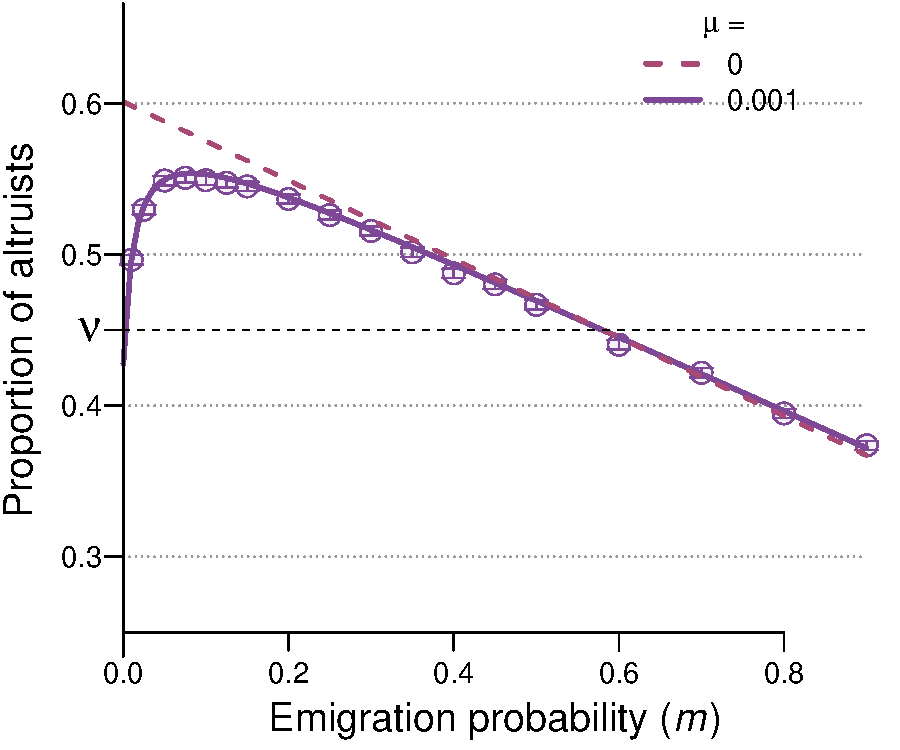
\includegraphics[width=\wpic]{{../../Programs/R/Pics/ESEB_EXDB_sel0.005_htg0_1}.pdf}};
}
\uncover<8>{
\node[]at(pM) (pMp){\includegraphics[width=\wpic]{{../../Programs/R/Pics/ESEB_EXDB_sel0.005_htg0_2}.pdf}};
}
\uncover<9>{
\node[]at(pM) (pMp){\includegraphics[width=\wpic]{{../../Programs/R/Pics/ESEB_EXDB_sel0.005_htg0_3}.pdf}};
}
\uncover<10>{
\node[]at(pM) (pMp){\includegraphics[width=\wpic]{{../../Programs/R/Pics/ESEB_EXDB_sel0.005_htg0_4}.pdf}};
}

\end{tikzpicture}

\btVFill
{\small ($b=15, c=1, \demesize = 4, \nbdemes = 15, \selstr = 0.005$)}
\end{center}

\end{frame}

\subsection{Robustness}

\begin{frame}

\begin{center}
{\LARGE \color{maincol} Is the result robust?}
\end{center}
\end{frame}

\begin{frame}{Another life-cycle}

\begin{center}

\begin{tikzpicture}
\uncover<2>{
\node[](pBD){\includegraphics[width=\wpic]{{../../Programs/R/Pics/ESEB_EXBD_sel0.005_htg0_justMu0}.pdf}
};
}

\node[above = 0cm of pBD]{Moran Birth-Death ($1$ birth \& $1$ death)};
\uncover<3>{\node[]at(pBD){\includegraphics[width=\wpic]{{../../Programs/R/Pics/ESEB_EXBD_sel0.005_htg0_leg}.pdf}
};
}
\end{tikzpicture}
\btVFill
{\small ($b=15, c=1, \demesize = 4, \nbdemes = 15, \selstr = 0.005$)}

\end{center}

\end{frame}

\begin{frame}{Strong selection}
\begin{center}

\begin{tikzpicture}

\uncover<1>{
\node[] (pWFs){\includegraphics[width=\wpic]{{../../Programs/R/Pics/ESEB_EXWF_sel0.005_htg0}.pdf}
};
\node[above= 0cm of pWFs]{Wright-Fisher, weak selection};


\node[right = 0cm of pWFs](pDBs){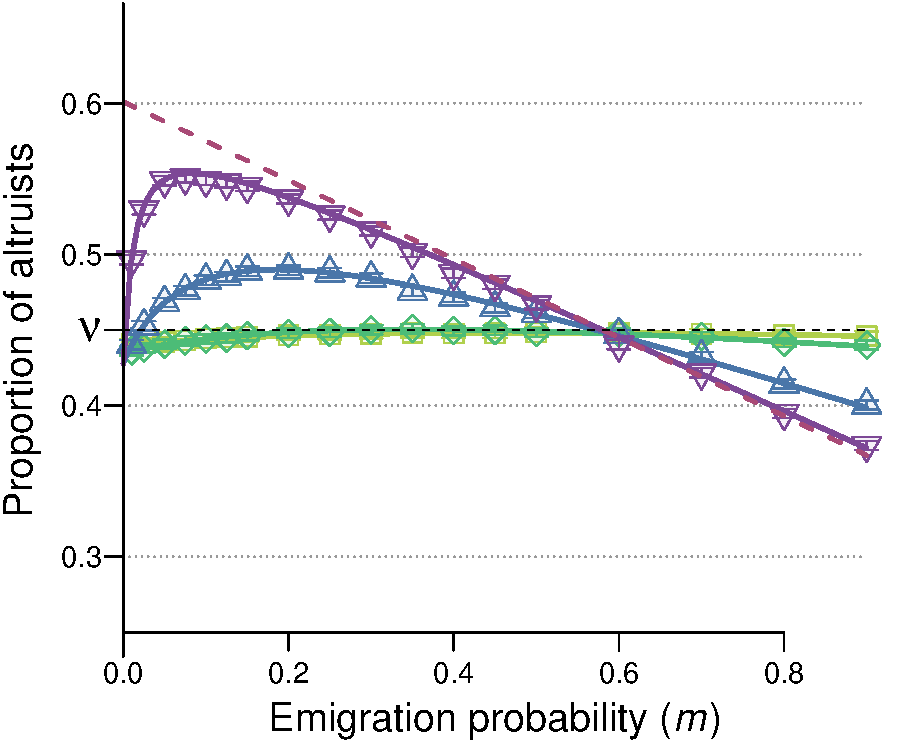
\includegraphics[width=\wpic]{{../../Programs/R/Pics/ESEB_EXDB_sel0.005_htg0}.pdf}
};
\node[above= 0cm of pDBs]{Moran Death-Birth, weak selection};
}

\uncover<2>{
\node[] (pWFs){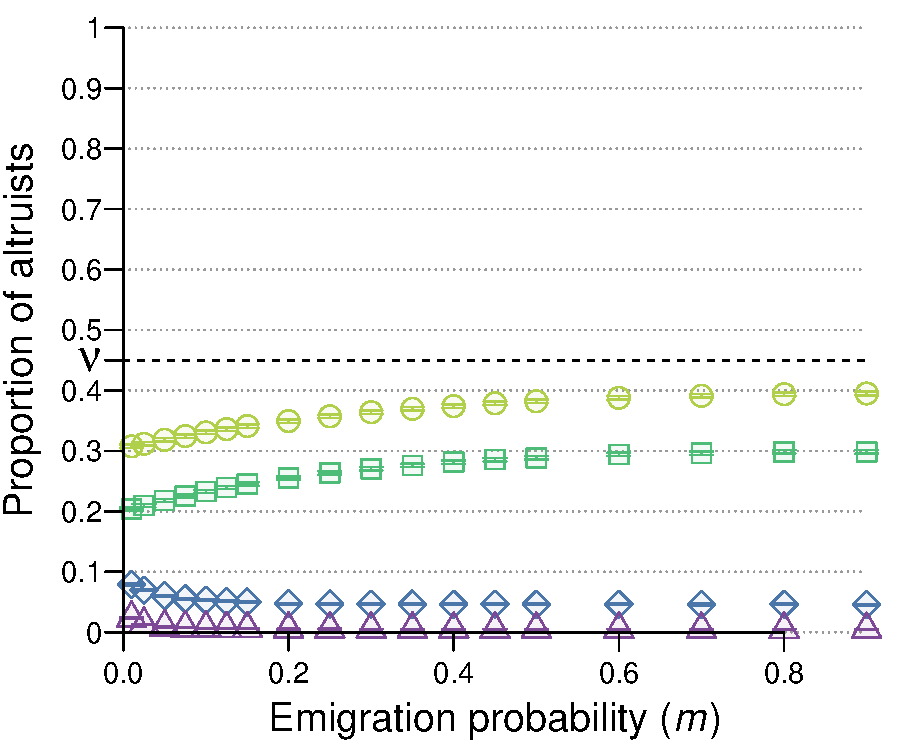
\includegraphics[width=\wpic]{{../../Programs/R/Pics/ESEB_EXWF_sel0.1_htg0}.pdf}
};
\node[above= 0cm of pWFs]{Wright-Fisher, strong selection};


\node[right = 0cm of pWFs](pDBs){\includegraphics[width=\wpic]{{../../Programs/R/Pics/ESEB_EXDB_sel0.1_htg0}.pdf}
};
\node[above= 0cm of pDBs]{Moran Death-Birth, strong selection};
}


\end{tikzpicture}
\alt<2>{\btVFill
{\small ($b=15, c=1, \demesize = 4, \nbdemes = 15, \selstr = 0.1$)}
}{\btVFill
{\small ($b=15, c=1, \demesize = 4, \nbdemes = 15, \selstr = 0.005$)}
}
\end{center}
\end{frame}


\begin{frame}{Heterogeneous deme sizes ($\overline{n} = 4$ as before, but $2\leq n \leq 5$)}
\begin{center}
\begin{tikzpicture}
\node[] (pWFs){\includegraphics[width=\wpic]{{../../Programs/R/Pics/ESEB_EXWF_sel0.005_htg1}.pdf}
};
\node[above= 0cm of pWFs]{Wright-Fisher};


\node[right = 0cm of pWFs](pDBs){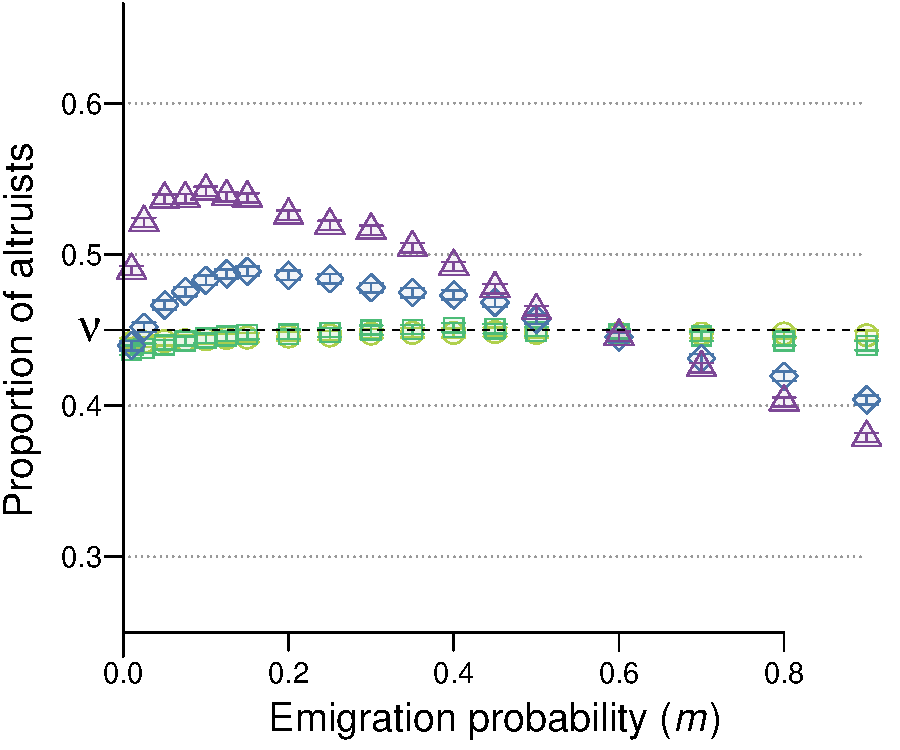
\includegraphics[width=\wpic]{{../../Programs/R/Pics/ESEB_EXDB_sel0.005_htg1}.pdf}
};
\node[above= 0cm of pDBs]{Moran Death-Birth};

\end{tikzpicture}
\btVFill
{\small ($b=15, c=1, \overline{\demesize} = 4, \nbdemes = 15, \selstr = 0.005$)}

\end{center}
\end{frame}


\begin{frame}{bfjdklf }
\includegraphics[width=0.5\textwidth]{{../../Programs/R/Pics/ESEB_EXWF_sel0.005_htg0_3}.pdf}
\end{frame}
\begin{frame}{bfjdklf }
fjdksl fjj fjkds lj
\end{frame}


\end{document}

